\chapter{Pianificazione del progetto}
\begin{redbar}
La \textbf{pianificazione del progetto} è uno dei compiti più importanti di un project manager nel settore software. Come manager, devi suddividere il lavoro in parti, assegnarle ai membri del team, anticipare i problemi che potrebbero sorgere e preparare soluzioni provvisorie per affrontarli. Il piano di progetto, creato all'inizio del progetto e aggiornato man mano che il progetto progredisce, serve a mostrare come verrà svolto il lavoro e a valutare l'andamento del progetto.
\end{redbar}

La pianificazione avviene in tre fasi principali durante il ciclo di vita di un progetto:
\begin{enumerate}
    \item \textit{Fase di proposta.} Durante la gara d'appalto per un contratto, è necessario elaborare un piano per decidere se si hanno le risorse per completare il lavoro e calcolare il prezzo da proporre al cliente.
    \item \textit{Fase di avvio del progetto.} Una volta ottenuto il contratto, si pianifica chi lavorerà al progetto, come suddividere il lavoro in incrementi e come allocare le risorse. \item \textit{Aggiornamenti periodici.} Durante il progetto, il piano viene aggiornato per riflettere le nuove informazioni acquisite sul software, il processo di sviluppo e il team di sviluppo.
\end{enumerate}
Nella fase di proposta, la pianificazione è inevitabilmente speculativa, poiché non si dispone di un set completo di requisiti per il software da sviluppare. Si risponde a una richiesta basata su una descrizione ad alto livello delle funzionalità richieste.
Un piano credibile è spesso richiesto come parte della proposta. Se il contratto viene assegnato, si deve ripianificare il progetto considerando eventuali cambiamenti e nuove informazioni emerse.

Durante la preparazione della proposta, è necessario calcolare il prezzo da proporre al cliente. Questo si basa sulla stima dei costi per completare il lavoro, considerando i seguenti parametri principali: costi di sforzo, costi hardware e software, costi di viaggio e formazione, costi indiretti...

Dopo l’assegnazione del contratto, il piano preliminare deve essere affinato per creare un piano di avvio dettagliato. Questo aiuta a prendere decisioni su budget e personale, allocare risorse e monitorare l'avanzamento del progetto. Il piano di avvio dovrebbe anche definire i meccanismi di monitoraggio del progetto. Anche nei metodi agili è necessario un piano iniziale per allocare risorse e stabilire le basi del progetto.

Il piano di progetto dovrebbe essere regolarmente aggiornato man mano che il progetto avanza e si acquisiscono maggiori informazioni sul software e sul suo sviluppo. Il programma del progetto, la stima dei costi e i rischi devono essere revisionati regolarmente.

\section{Prezzi del software}
In linea di principio, il prezzo di un sistema software sviluppato per un cliente corrisponde semplicemente al costo dello sviluppo più il profitto per il fornitore. Tuttavia, in pratica, la relazione tra il costo del progetto e il prezzo proposto al cliente non è quasi mai così semplice. Nel calcolo di un prezzo, si devono considerare fattori organizzativi, economici, politici e commerciali più ampi (Tabella \ref{tab:factors-software-pricing}). Questi aspetti possono portare ad un adeguamento del prezzo verso l’alto o verso il basso.

\begin{table}[ht]
\centering
\rowcolors{2}{lightblue}{lightgray}
\begin{tabular}{|p{3.5cm}|p{11cm}|}
\hline
\rowcolor{headerblue}
\textbf{\textcolor{white}{Fattore}} & \textbf{\textcolor{white}{Descrizione}} \\\hline
Termini contrattuali & Un cliente potrebbe consentire al sviluppatore di mantenere la proprietà del codice sorgente e riutilizzarlo in altri progetti. In questo caso, il prezzo richiesto potrebbe essere inferiore rispetto alla consegna del codice sorgente al cliente.\\\hline
Incertezza nella stima dei costi & Se un'organizzazione non è sicura della stima dei costi, potrebbe aumentare il prezzo aggiungendo una percentuale di contingenza oltre al normale margine di profitto.\\\hline
Salute finanziaria & Gli sviluppatori in difficoltà finanziarie potrebbero abbassare il prezzo per ottenere un contratto. È preferibile ottenere un profitto inferiore al normale o andare in pareggio piuttosto che uscire dal mercato. In tempi difficili, il flusso di cassa è più importante del profitto.\\\hline
Opportunità di mercato & Un'organizzazione di sviluppo potrebbe offrire un prezzo basso per entrare in un nuovo segmento di mercato software. Accettare un basso profitto su un progetto può dare l'opportunità di ottenere profitti maggiori in futuro. L'esperienza acquisita potrebbe anche aiutare a sviluppare nuovi prodotti.\\\hline
Volatilità dei requisiti & Se i requisiti potrebbero cambiare, un'organizzazione può abbassare il prezzo per aggiudicarsi il contratto. Dopo l'assegnazione, possono essere applicati prezzi più alti per le modifiche ai requisiti.
\\\hline
\end{tabular}
\caption{Fattori che influenzano il prezzo del software}
\label{tab:factors-software-pricing}
\end{table}

Esistono due tipologie di strategie di prezzo:
\begin{enumerate}
    \item \textit{Prezzo al ribasso.} Un'azienda può offrire un prezzo inferiore per aggiudicarsi un contratto che consenta di mantenere il personale per opportunità future. Un'azienda può offrire un prezzo inferiore per accedere a un nuovo segmento di mercato.
    \item \textit{Prezzo aumentato.} Il prezzo può essere aumentato quando l'acquirente richiede un contratto a prezzo fisso, e il venditore incrementa il prezzo per coprire eventuali rischi imprevisti.
\end{enumerate}
Il pricing to win implica che un'azienda abbia un'idea del prezzo che il cliente si aspetta di pagare e prepari un'offerta per il contratto basata su tale aspettativa. 
Un costo di progetto viene concordato sulla base di una proposta preliminare. Successivamente, si avviano negoziazioni tra cliente e fornitore per definire le specifiche dettagliate del progetto.

\section{Sviluppo plan-driven}
Lo sviluppo basato su piani (plan-driven) è un approccio all'ingegneria del software in cui il processo di sviluppo viene pianificato in dettaglio. Viene creato un piano di progetto che registra il lavoro da svolgere, chi lo eseguirà, il programma di sviluppo e i prodotti finali. I responsabili utilizzano il piano per supportare le decisioni relative al progetto e per misurare i progressi. Lo sviluppo plan-driven si basa su tecniche di gestione dei progetti ingegneristici ed è considerato il metodo "tradizionale" per gestire grandi progetti di sviluppo software. Lo sviluppo agile, al contrario, utilizza un processo di pianificazione diverso, in cui le decisioni vengono posticipate.

Il problema dello sviluppo plan-driven è che le decisioni prese in anticipo devono spesso essere riviste a causa di cambiamenti negli ambienti in cui il software viene sviluppato e utilizzato. Ritardare le decisioni di pianificazione può evitare inutili rifacimenti. Tuttavia, i vantaggi di un approccio plan-driven sono che una pianificazione anticipata consente di tenere conto di questioni organizzative (disponibilità del personale, altri progetti, ecc.). Problemi e dipendenze potenziali vengono scoperti prima che il progetto inizi, piuttosto che quando il progetto è già avviato.

\subsection{Piani di progetto}
In un progetto di sviluppo plan-driven, il piano del progetto stabilisce le risorse disponibili, la suddivisione del lavoro e un programma per l'esecuzione delle attività. I dettagli dei piani di progetto variano in base al tipo di progetto e organizzazione, ma in genere includono le seguenti sezioni:
\begin{enumerate}    
    \item \textit{Introduzione.} Descrive brevemente gli obiettivi del progetto e stabilisce i vincoli (ad esempio, budget, tempi) che influenzano la gestione del progetto.
    \item \textit{Organizzazione del progetto.} Descrive il modo in cui il team di sviluppo è organizzato, le persone coinvolte e i loro ruoli all'interno del team.
    \item \textit{Analisi dei rischi.} Descrive i possibili rischi del progetto, la probabilità che si verifichino e le strategie di riduzione del rischio che vengono proposte.
    \item \textit{Requisiti di risorse hardware e software.} Specifica l'hardware e il software di supporto necessari per eseguire lo sviluppo. Se è necessario acquistare hardware, possono essere incluse stime sui prezzi e sul programma di consegna.
    \item \textit{Suddivisione del lavoro.} Definisce la suddivisione del progetto in attività e identifica gli input e gli output di ciascuna attività del progetto.
    \item \textit{Pianificazione del progetto.} Mostra le dipendenze tra le attività, il tempo stimato per raggiungere ogni traguardo e l'assegnazione del personale alle attività.
    \item \textit{Meccanismi di monitoraggio e reporting.} Definisce i report di gestione da produrre, quando devono essere prodotti e i meccanismi di monitoraggio del progetto da utilizzare.
\end{enumerate}
Il piano principale del progetto dovrebbe sempre includere una valutazione dei rischi e un programma del progetto. Inoltre, potrebbero essere sviluppati piani supplementari per attività specifiche (Tabella \ref{tab:project-plan-supplements}).

\begin{table}[ht]
\centering
\rowcolors{2}{lightblue}{lightgray}
\begin{tabular}{|p{4cm}|p{10.5cm}|}
\hline
\rowcolor{headerblue}
\textbf{\textcolor{white}{Piano}} & \textbf{\textcolor{white}{Descrizione}} \\\hline
Piano di gestione delle configurazioni & Descrive le procedure e le strutture di gestione delle configurazioni che saranno utilizzate.\\\hline
Piano di distribuzione & Descrive come il software e l'hardware associato (se richiesto) saranno distribuiti nell'ambiente del cliente. Questo dovrebbe includere un piano per la migrazione dei dati dai sistemi esistenti.\\\hline
Piano di manutenzione & Prevede i requisiti, i costi e l'impegno necessari per la manutenzione.\\\hline
Piano di qualità & Descrive le procedure e gli standard di qualità che saranno utilizzati in un progetto.\\\hline
Piano di validazione & Descrive l'approccio, le risorse e il programma utilizzati per la validazione del sistema.
\\\hline
\end{tabular}
\caption{Supplementi al piano di progetto}
\label{tab:project-plan-supplements}
\end{table}

\subsection{Il processo di pianificazione}
La pianificazione del progetto è un processo iterativo che inizia con la creazione di un piano iniziale durante la fase di avvio del progetto.

Le modifiche al piano sono inevitabili. Man mano che si ottengono maggiori informazioni sul sistema e sul team di progetto, è necessario rivedere regolarmente il piano per riflettere i cambiamenti nei requisiti, nella pianificazione e nei rischi. Anche la modifica degli obiettivi aziendali comporta modifiche nei piani di progetto. Man mano che gli obiettivi aziendali cambiano, ciò potrebbe influire su tutti i progetti, che potrebbero quindi dover essere ripianificati.

\begin{figure}[ht]
    \centering
    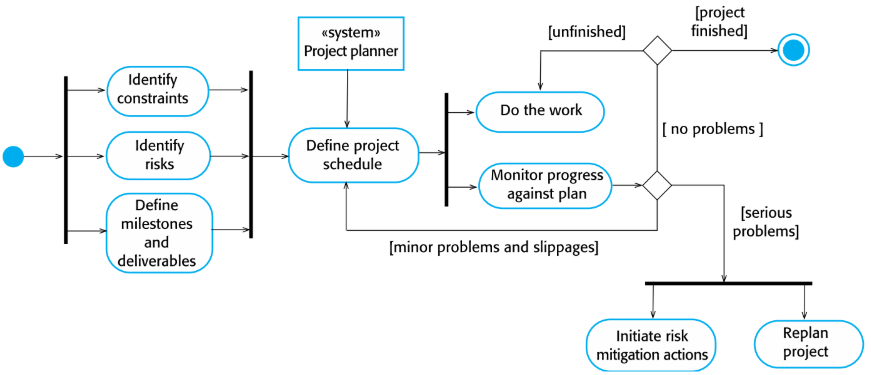
\includegraphics[width=0.80\linewidth]{images/project-planning-process.PNG}
    \caption{Il processo di pianificazione del progetto}
    \label{fig:project-planning-process}
\end{figure}

All'inizio del processo di pianificazione, si dovrebbero valutare i vincoli che influenzano il progetto, come la data di consegna richiesta, il personale disponibile, il budget complessivo e gli strumenti disponibili. Bisogna anche identificare i traguardi e i prodotti da consegnare.

Il processo entra quindi in un ciclo che termina solo quando il progetto è completato. Durante questo ciclo, si redige un programma stimato, si avviano le attività definite e si rivedono regolarmente i progressi.

Se emergono seri problemi che potrebbero causare ritardi significativi, è necessario adottare azioni di mitigazione del rischio per ridurre il rischio di fallimento del progetto. Se queste azioni non sono efficaci, è opportuno avviare una revisione tecnica formale del progetto, che può anche portare alla decisione di annullare il progetto se non è più allineato agli obiettivi aziendali.

È importante fare ipotesi realistiche piuttosto che ottimistiche durante la definizione di un piano di progetto. Durante un progetto sorgono sempre problemi di qualche tipo, che portano a ritardi nello sviluppo. Pertanto, le ipotesi iniziali e la pianificazione devono tenere conto di problemi imprevisti. Bisogna includere una contingenza nel piano per evitare che eventuali problemi compromettano gravemente la scadenza di consegna. 

Se si verificano problemi significativi nello sviluppo che potrebbero causare ritardi considerevoli, è necessario avviare azioni di mitigazione del rischio per ridurre i rischi di fallimento del progetto. In parallelo a queste azioni, bisogna anche ripianificare il progetto.
Questo potrebbe comportare la rinegoziazione dei vincoli e delle consegne del progetto con il cliente. Bisogna stabilire e concordare con il cliente un nuovo programma per il completamento delle attività.

\section{Pianificazione del progetto}
La pianificazione del progetto è il processo di definizione di come il lavoro in un progetto sarà organizzato in compiti separati, e quando e come questi compiti saranno eseguiti. Devi stimare il tempo necessario per completare ogni compito e l'impegno richiesto, suggerendo chi lavorerà sui compiti identificati. Devi anche stimare le risorse hardware e software necessarie per completare ciascun compito. Ad esempio, se stai sviluppando un sistema embedded, devi stimare il tempo necessario per utilizzare hardware specializzato e i costi per eseguire un simulatore di sistema. 

Sia i processi basati su piano che quelli agili richiedono una pianificazione iniziale del progetto. Questa pianificazione iniziale viene utilizzata per pianificare come le persone saranno allocate ai progetti e per verificare i progressi del progetto rispetto agli impegni contrattuali.

La pianificazione nei progetti basati su piano (Figura \ref{fig:project-scheduling-process}) implica suddividere il lavoro totale di un progetto in compiti separati e stimare il tempo necessario per completare ciascun compito. I compiti dovrebbero normalmente durare almeno una settimana e non più di 2 mesi. Una suddivisione più fine comporta un dispendio di tempo sproporzionato per la ripianificazione e l'aggiornamento del piano di progetto. Il tempo massimo per ciascun compito dovrebbe essere di 6-8 settimane. Se un compito richiede più tempo, dovrebbe essere suddiviso in sottocompiti per la pianificazione e la schedulazione del progetto.

\begin{figure}[ht]
    \centering
    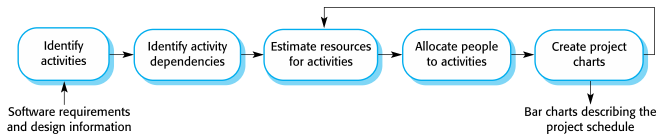
\includegraphics[width=0.75\linewidth]{images/project-scheduling-process.PNG}
    \caption{Il processo di pianificazione del progetto}
    \label{fig:project-scheduling-process}
\end{figure}

Alcuni di questi compiti vengono eseguiti in parallelo, con persone diverse che lavorano su componenti differenti del sistema. Devi coordinare questi compiti paralleli e organizzare il lavoro in modo che la forza lavoro venga utilizzata in modo ottimale e che non vengano introdotte dipendenze inutili tra i compiti. È importante evitare una situazione in cui l'intero progetto venga ritardato a causa del fatto che un compito critico non è stato completato.

Se un progetto è tecnicamente avanzato, le stime iniziali saranno quasi certamente ottimistiche anche quando si cercherà di considerare tutte le eventualità. Le pianificazioni, quindi, devono essere continuamente aggiornate man mano che diventano disponibili informazioni più precise sui progressi.

Stimare la difficoltà dei problemi e quindi il costo per sviluppare una soluzione è difficile. La produttività non è proporzionale al numero di persone che lavorano su un compito. Aggiungere persone a un progetto in ritardo lo rende ancora più in ritardo a causa dei costi di comunicazione. Quando si stima la pianificazione, è necessario tenere in considerazione la possibilità che qualcosa vada storto e prevedere una contingenza nella pianificazione.

\subsection{Presentazione della pianificazione}
Sono stati sviluppati dei grafici alternativi per visualizzare le pianificazioni del progetto, che sono spesso più facili da leggere e comprendere. Due tipi di visualizzazione sono comunemente utilizzati:
\begin{enumerate}
    \item Grafici a barre basati sul calendario mostrano chi è responsabile di ciascuna attività, il tempo previsto, e quando l'attività è programmata per iniziare e finire.
    \item Reti di attività mostrano le dipendenze tra le diverse attività che compongono un progetto.
\end{enumerate}
Le attività di progetto sono l'elemento base della pianificazione. Ogni attività ha:
\begin{itemize}
    \item una durata in giorni o mesi di calendario;
    \item una stima dell’impegno, che mostra il numero di giorni persona o mesi persona necessari per completare il lavoro;
    \item una scadenza entro la quale l’attività deve essere completata;
    \item un punto finale definito, che potrebbe essere un documento, la tenuta di una riunione di revisione, l’esecuzione con successo di tutti i test, e così via.
\end{itemize}

Quando si pianifica un progetto, si potrebbe decidere di definire delle tappe (milestones). Una tappa è una fine logica di una fase del progetto, dove il progresso del lavoro può essere rivisto. Le tappe possono essere associate a un singolo compito o a gruppi di attività correlate.

Alcune attività creano deliverables di progetto, ossia risultati che vengono consegnati al cliente del software. Di solito, i deliverables richiesti sono specificati nel contratto di progetto, e la visione del cliente sul progresso del progetto dipende da questi deliverables. 

\begin{table}[ht]
\centering
\rowcolors{2}{lightblue}{lightgray}
\begin{tabular}{|c|c|c|c|}
\hline
\rowcolor{headerblue}
\textbf{\textcolor{white}{Task}} & \textbf{\textcolor{white}{Effort (person-days)}} & \textbf{\textcolor{white}{Duration (days)}} & \textbf{\textcolor{white}{Dependencies}} \\\hline
T1 & 15 & 10 & \\\hline
T2 & 8 & 15 & \\\hline
T3 & 20 & 15 & T1 (M1)\\\hline
T4 & 5 & 10 & \\\hline
T5 & 5 & 10 & T2, T4 (M3)\\\hline
T6 & 10 & 5 & T1, T2 (M4)\\\hline
T7 & 25 & 20 & T1 (M1)\\\hline
T8 & 75 & 25 & T4 (M2)\\\hline
T9 & 10 & 15 & T3, T6 (M5)\\\hline
T10 & 20 & 15 & T7, T8 (M6)\\\hline
T11 & 10 & 10 & T9 (M7)\\\hline
T12 & 20 & 10 & T10, T11 (M8)
\\\hline
\end{tabular}
\caption{Attività, durate e dipendenze}
\label{tab:tasks-durations-dependencies}
\end{table}

Da questa tabella, si può vedere che il compito $T3$ dipende dal compito $T1$. Ciò significa che il compito $T1$ deve essere completato prima che $T3$ inizi.

Si noti che la durata stimata di alcuni compiti è maggiore rispetto all'impegno richiesto e viceversa. Se l’impegno è inferiore alla durata, le persone allocate a quel compito non stanno lavorando a tempo pieno su di esso. Se l’impegno è maggiore della durata, significa che più membri del team stanno lavorando contemporaneamente sul compito.

La Figura \ref{fig:activity-bar-chart} prende le informazioni della Tabella \ref{tab:tasks-durations-dependencies} e presenta la pianificazione del progetto come un grafico a barre che mostra il calendario del progetto e le date di inizio e fine dei compiti. Leggendo da sinistra a destra, il grafico a barre mostra chiaramente quando i compiti iniziano e finiscono. Le tappe ($M1$, $M2$, ecc.) sono anche mostrate nel grafico a barre. Si noti che i compiti che sono indipendenti possono essere eseguiti in parallelo. Ad esempio, i compiti $T1$, $T2$ e $T4$ iniziano all'inizio del progetto.

\begin{figure}[ht]
    \centering
    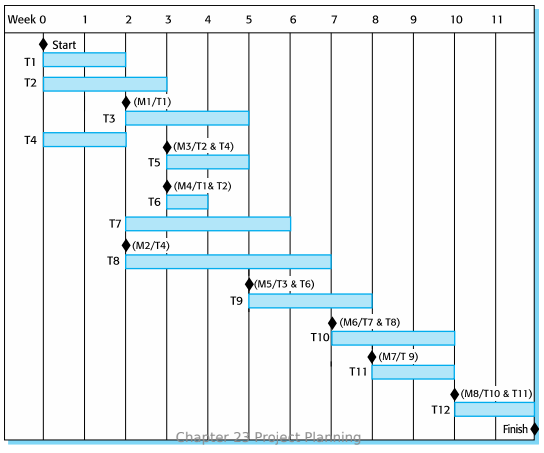
\includegraphics[width=0.65\linewidth]{images/activity-bar-chart.PNG}
    \caption{Grafico a barre delle attività}
    \label{fig:activity-bar-chart}
\end{figure}

Oltre a pianificare la programmazione di consegna del software, i project manager devono allocare risorse ai compiti. La risorsa chiave è, ovviamente, l’ingegnere del software che eseguirà il lavoro. Devono essere assegnati alle attività di progetto. L'allocazione delle risorse può essere analizzata utilizzando strumenti di gestione del progetto, e un grafico a barre può essere generato per mostrare quando il personale sta lavorando sul progetto (Figura \ref{fig:staff-allocation-chart}). Le persone possono lavorare su più di un compito contemporaneamente e, a volte, non lavorano sul progetto. Possono essere in ferie, lavorare su altri progetti o partecipare a corsi di formazione. Gli incarichi part-time vengono mostrati utilizzando una linea diagonale che attraversa la barra.

\begin{figure}[ht]
    \centering
    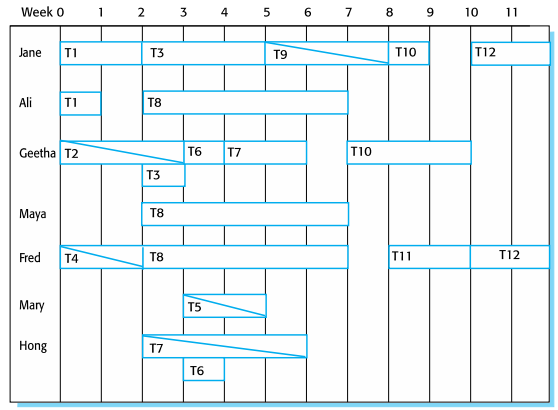
\includegraphics[width=0.6\linewidth]{images/staff-allocation-chart.PNG}
    \caption{Tabella di allocazione del personale}
    \label{fig:staff-allocation-chart}
\end{figure}

Se un compito subisce un ritardo, i compiti successivi che dipendono da esso possono essere influenzati. Non possono iniziare fino a quando il compito ritardato non viene completato. 

\section{Pianificazione agile}
I metodi agili di sviluppo software sono approcci iterativi in cui il software viene sviluppato e consegnato ai clienti in incrementi. A differenza degli approcci plan-driven, la funzionalità di questi incrementi non viene pianificata in anticipo ma viene decisa durante lo sviluppo. La decisione su cosa includere in un incremento dipende dai progressi e dalle priorità del cliente. L'argomentazione a favore di questo approccio è che le priorità e i requisiti del cliente cambiano, quindi ha senso avere un piano flessibile che possa adattarsi a tali cambiamenti.

I metodi di sviluppo agile come Scrum e Extreme Programming adottano un approccio alla pianificazione in due fasi, corrispondenti alla fase di avvio e alla pianificazione dello sviluppo nei metodi tradizionali:
\begin{enumerate}
    \item Pianificazione del rilascio, che guarda avanti per diversi mesi e decide quali funzionalità includere in un rilascio del sistema.
    \item Pianificazione dell'iterazione, che ha un orizzonte temporale più breve e si concentra sulla pianificazione del prossimo incremento del sistema, solitamente rappresentando 2-4 settimane di lavoro per il team.
\end{enumerate}
L'approccio Scrum alla pianificazione, basato su backlog di progetto e revisioni quotidiane del lavoro da fare. Questo approccio è principalmente orientato alla pianificazione delle iterazioni. Un altro approccio alla pianificazione agile, sviluppato come parte di Extreme Programming, si basa sulle user stories. Il cosiddetto planning game può essere utilizzato sia per la pianificazione del rilascio sia per quella delle iterazioni.

\begin{figure}[ht]
    \centering
    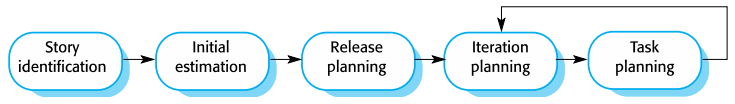
\includegraphics[width=0.65\linewidth]{images/planning-game.PNG}
    \caption{Il planning game}
    \label{fig:planning-game}
\end{figure}

La base del planning game (Figura \ref{fig:planning-game}) è un insieme di user stories che coprono tutte le funzionalità da includere nel sistema finale. Il team di sviluppo e il cliente lavorano insieme per sviluppare queste storie. I membri del team leggono e discutono le storie e le classificano in base al tempo necessario per implementarle. Alcune storie possono essere troppo grandi per essere implementate in una sola iterazione e vengono quindi suddivise in storie più piccole.

Poiché stimare lo sforzo o il tempo necessario può essere difficile, viene spesso utilizzata una classificazione relativa. Il team confronta le storie a coppie e decide quale richiederà più tempo ed effort, senza valutare esattamente quanto sarà necessario. Alla fine di questo processo, l'elenco delle storie è ordinato, con le storie più complesse in cima alla lista. Il team assegna quindi dei punti effort a tutte le storie: ad esempio, una storia complessa potrebbe ricevere 8 punti, una semplice 2 punti.

Una volta stimate le storie, l'effort relativo viene tradotto in una prima stima dello sforzo totale richiesto usando il concetto di velocità (velocity), ovvero il numero di punti effort implementati dal team al giorno. Questo dato può essere stimato dall'esperienza precedente o implementando una o due storie per verificare quanto tempo serve. Con una stima della velocità, si può calcolare lo sforzo totale in giorni/persona per implementare il sistema.

La pianificazione del rilascio implica la selezione e il perfezionamento delle storie che riflettono le funzionalità da implementare in un rilascio del sistema, nonché l'ordine di implementazione.

Le storie da implementare durante l'iterazione vengono scelte in base al tempo disponibile (solitamente 2-3 settimane) e alla velocità del team. Alla fine dell'iterazione, anche se non tutte le storie sono state implementate, l'incremento viene considerato completo. La velocità viene ricalcolata e utilizzata per pianificare la versione successiva.

All'inizio di ogni iterazione, c'è una fase di pianificazione dei compiti in cui gli sviluppatori suddividono le storie in task di sviluppo. Un task dovrebbe richiedere tra 4 e 16 ore. Gli sviluppatori scelgono i task che implementeranno, sapendo la propria velocità individuale, così da non accettare più compiti di quelli che possono completare.

Questo approccio alla pianificazione ha due vantaggi principali:
\begin{enumerate}
    \item Il team ha una panoramica dei task da completare, comprendendo chi sta facendo cosa e facilitando la collaborazione.
    \item Gli sviluppatori scelgono i propri compiti, aumentando il senso di proprietà e la motivazione.
\end{enumerate}
Un incremento di software viene sempre consegnato alla fine di ogni iterazione, e se le funzionalità non possono essere completate, il lavoro viene ridotto senza estendere la scadenza. Tuttavia, ciò può creare problemi ai clienti, poiché devono utilizzare un sistema incompleto o modificare i propri processi.

La pianificazione agile funziona bene con team piccoli e stabili. Tuttavia, nei grandi progetti, con team distribuiti geograficamente o in cui i membri cambiano spesso, è difficile attuare la collaborazione necessaria. In questi casi, si utilizzano approcci tradizionali alla gestione del progetto.

\section{Tecniche di stima}
Stimare i tempi di un progetto è un compito difficile. Ci sono così tante incertezze che è impossibile stimare accuratamente i costi di sviluppo del sistema nelle prime fasi di un progetto. Tuttavia, le organizzazioni devono comunque effettuare stime di sforzo e costo. Per farlo, possono essere utilizzate due tipi di tecniche:
\begin{enumerate}
    \item \textit{Tecniche basate sull'esperienza.} La stima delle future esigenze di sforzo si basa sull'esperienza del responsabile di progetto relativa a progetti passati e al dominio applicativo. Essenzialmente, il manager formula un giudizio informato sulle probabili necessità di sforzo.
    \item \textit{Modelli algoritmici di costo.} In questo approccio, si utilizza una formula per calcolare lo sforzo del progetto basandosi su stime di attributi del prodotto, come dimensioni, caratteristiche del processo e competenze del personale coinvolto.
\end{enumerate}
In entrambi i casi, è necessario utilizzare il proprio giudizio per stimare direttamente lo sforzo oppure le caratteristiche del progetto e del prodotto. Nella fase iniziale di un progetto, queste stime hanno un ampio margine di errore. Se la stima iniziale dello sforzo richiesto è di $x$ mesi di lavoro, il range effettivo potrebbe variare da $0,25x$ a $4x$ rispetto allo sforzo reale misurato al completamento del sistema. Durante la pianificazione dello sviluppo, le stime diventano progressivamente più accurate man mano che il progetto avanza (Figura \ref{fig:estimate-uncertainty}).

\begin{figure}[ht]
    \centering
    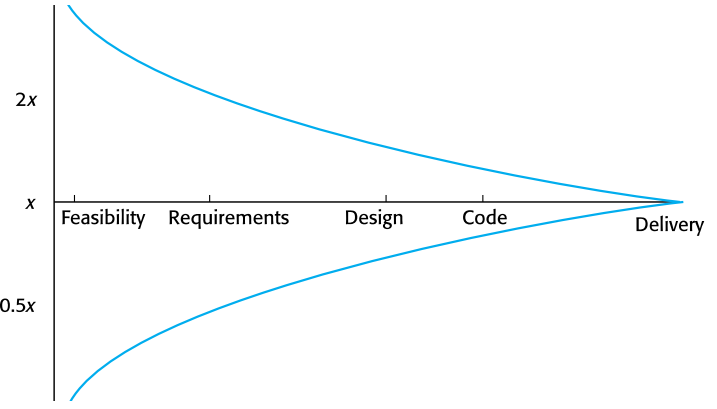
\includegraphics[width=0.55\linewidth]{images/estimate-uncertainty.PNG}
    \caption{Stima dell'incertezza}
    \label{fig:estimate-uncertainty}
\end{figure}

\subsection{Tecniche basate sull'esperienza}
Le tecniche basate sull'esperienza si basano sull'esperienza del manager relativa a progetti passati e sullo sforzo effettivamente impiegato in tali progetti per attività correlate allo sviluppo software. Tipicamente, si identificano i deliverable da produrre in un progetto e i diversi componenti o sistemi software da sviluppare. Questi vengono documentati in un foglio di calcolo, stimati individualmente e poi sommati per calcolare lo sforzo totale richiesto. Coinvolgere un gruppo di persone nell'attività di stima può essere utile: ogni membro del gruppo spiega la propria stima, rivelando spesso fattori che altri non avevano considerato, permettendo di iterare fino a ottenere una stima condivisa.

La difficoltà con le tecniche basate sull'esperienza è che un nuovo progetto software potrebbe non avere molto in comune con progetti precedenti. Lo sviluppo software cambia molto rapidamente, e un progetto potrebbe spesso utilizzare tecniche non familiari come i servizi web, la configurazione di sistemi applicativi o HTML5. Se non si ha esperienza con queste tecniche, l'esperienza passata potrebbe non aiutare a stimare lo sforzo richiesto, rendendo più difficile produrre stime accurate di costi e tempi.

\subsection{Modelli algoritmici di costo}
La modellazione algoritmica dei costi utilizza una formula matematica per prevedere i costi di progetto basandosi su stime delle dimensioni del progetto, del tipo di software da sviluppare e di altri fattori legati al team, al processo e al prodotto.

La maggior parte dei modelli algoritmici per stimare lo sforzo in un progetto software si basa su una formula semplice:
\begin{equation*}
    Effort = A\times Size^B\times M
\end{equation*}
$A$: un fattore costante che dipende dalle pratiche organizzative locali e dal tipo di software sviluppato. $Size$: una valutazione delle dimensioni del codice del software o una stima della funzionalità espressa in function points o application points. $B$: rappresenta la complessità del software e solitamente varia tra 1 e 1,5. $M$: un fattore che considera attributi di processo, prodotto e sviluppo, come i requisiti di affidabilità del software e l'esperienza del team di sviluppo.

Diversi fattori influenzano la dimensione finale: utilizzo di sistemi e componenti riutilizzati; linguaggio di programmazione; distribuzione del sistema. Man mano che il processo di sviluppo procede, la stima della dimensione diventa più accurata.

I modelli algoritmici dei costi rappresentano un modo sistematico per stimare lo sforzo necessario per sviluppare un sistema. Tuttavia, questi modelli sono complessi e difficili da utilizzare. Esistono molti attributi e un ampio margine di incertezza nella stima dei loro valori. Questa complessità limita l'applicazione pratica della modellazione algoritmica dei costi a un numero relativamente piccolo di grandi aziende, principalmente nei settori della difesa e dell'ingegneria aerospaziale.

\section{Modellazione dei costi COCOMO}
Questo modello empirico è stato sviluppato raccogliendo dati da un gran numero di progetti software di diverse dimensioni. I dati sono stati analizzati per scoprire le formule che meglio si adattavano alle osservazioni.

COCOMO II è un modello disponibile gratuitamente ed è supportato da strumenti open-source.

COCOMO II è stato sviluppato a partire dai precedenti modelli di stima dei costi COCOMO (Constructive Cost Modeling), basati principalmente sullo sviluppo di codice originale. Il modello COCOMO II tiene conto degli approcci moderni allo sviluppo software, come lo sviluppo rapido con linguaggi dinamici, lo sviluppo basato sul riuso e la programmazione di database. COCOMO II integra diversi sottomodelli basati su queste tecniche, che producono stime sempre più dettagliate.

I sottomodelli (Figura \ref{fig:cocomo-esitmation-models}) che fanno parte del modello COCOMO II sono:

\begin{figure}[ht]
    \centering
    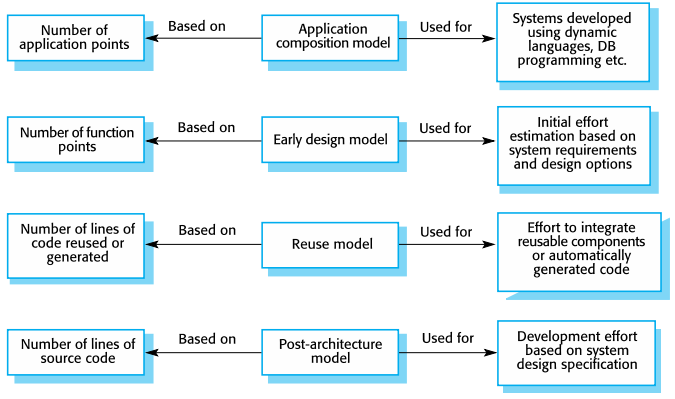
\includegraphics[width=0.65\linewidth]{images/cocomo-esitmation-models.PNG}
    \caption{Modelli di stima COCOMO}
    \label{fig:cocomo-esitmation-models}
\end{figure}
\begin{enumerate}
    \item \textit{Modello di composizione dell'applicazione.} Questo modello stima lo sforzo necessario per sviluppare sistemi creati da componenti riutilizzabili, scripting o programmazione di database.
    \textit{Modello per la progettazione preliminare.} Utilizzato nelle fasi iniziali della progettazione del sistema, dopo che i requisiti sono stati stabiliti.
    \textit{Modello di riuso.} Questo modello calcola lo sforzo necessario per integrare componenti riutilizzabili e/o codice generato automaticamente.
    \textit{Modello post-architettura.} Una volta progettata l'architettura del sistema, è possibile effettuare una stima più accurata delle dimensioni del software.
\end{enumerate}

\subsection{Modello di composizione dell'applicazione}
Il modello di composizione dell'applicazione è stato introdotto in COCOMO II per supportare la stima dello sforzo richiesto nei progetti di prototipazione e nei progetti in cui il software viene sviluppato componendo componenti esistenti. Si basa su una stima dei weighted application points (a volte chiamati object points), divisi per una stima standard della produttività in termini di application points.

La formula finale per calcolare lo sforzo richiesto per i prototipi di sistema è:
\begin{equation*}
    PM = (NAP\times(1-\%reuse/100))/PROD
\end{equation*}
Dove: $PM$ stima dello sforzo in person-months (mesi/uomo); $NAP$ è il numero totale di application points nel sistema consegnato; $\%reuse$ è la percentuale stimata di codice riutilizzato nello sviluppo; $PROD$ è la produttività degli application points, come mostrato nella Tabella \ref{tab:application-point-productivity}.

\begin{table}[ht]
\centering
\rowcolors{2}{lightblue}{lightgray}
\begin{tabular}{|l|l|l|l|l|l|}
\hline
\rowcolor{headerblue}
\textbf{\textcolor{white}{Esperienza e capacità dello sviluppatore}} & \textbf{\textcolor{white}{Molto bassa}} & \textbf{\textcolor{white}{Bassa}} & \textbf{\textcolor{white}{Nominale}} & \textbf{\textcolor{white}{Alta}} & \textbf{\textcolor{white}{Molto alta}} \\\hline
Maturità e capacità degli strumenti ICASE & Molto bassa & Bassa & Nominale & Alta & Molto alta\\\hline
PROD (NAP/mese) & 4 & 7 & 13 & 25 & 50
\\\hline
\end{tabular}
\caption{Attività, durate e dipendenze}
\label{tab:application-point-productivity}
\end{table}

\subsection{Modello di progettazione preliminare}
Si presume che i requisiti degli utenti siano stati concordati e che le fasi iniziali del processo di progettazione del sistema siano in corso. L'obiettivo a questo stadio è fornire una stima approssimativa e rapida dei costi. 

Le stime preliminari sono particolarmente utili per esplorare diverse opzioni, in modo da confrontare differenti modalità di implementazione dei requisiti dell'utente. Le stime prodotte in questa fase si basano sulla formula standard dei modelli algoritmici, ovvero:
\begin{equation*}
    PM=A\times Size^B\times M
\end{equation*}
$M = PERS\times RCPX\times RUSE\times PDIF\times PREX\times FCIL\times SCED$; $A$ è pari a 2,94, la dimensione del sistema viene espressa in KSLOC (migliaia di linee di codice sorgente); l'esponente $B$ riflette lo sforzo aggiuntivo necessario con l'aumentare della dimensione del progetto. Questo valore può variare da 1,1 a 1,24, a seconda della novità del progetto, della flessibilità dello sviluppo, dei processi di gestione dei rischi, della coesione del team di sviluppo e del livello di maturità dei processi dell'organizzazione.

Il moltiplicatore $M$ si basa su sette attributi del progetto e del processo che possono aumentare o diminuire la stima.
\begin{itemize}
    \item $PERS$: capacità del personale
    \item $PREX$: esperienza del personale
    \item $RCPX$: affidabilità e complessità del prodotto
    \item $RUSE$: riuso richiesto
    \item $PDIF$: difficoltà della piattaforma
    \item $SCED$: programmazione temporale
    \item $FSIL$: strutture di supporto
\end{itemize}

\subsection{Modello di riuso}
Il modello di riuso COCOMO viene utilizzato per stimare lo sforzo necessario per integrare codice riutilizzabile o generato automaticamente.

COCOMO II considera due tipi di codice riutilizzato:
\begin{enumerate}
    \item \textit{Codice a scatola nera (black-box)}: è codice riutilizzabile senza necessità di comprenderlo o modificarlo. Lo sforzo di sviluppo per il codice black-box è considerato pari a zero, e la sua dimensione non è inclusa nel calcolo complessivo dello sforzo.
    \item \textit{Codice a scatola bianca (white-box)}: è codice riutilizzabile che deve essere adattato per integrarsi con il nuovo codice o con altri componenti riutilizzati. Questo richiede uno sforzo aggiuntivo per comprendere e modificare il codice affinché funzioni correttamente nel sistema in sviluppo.
\end{enumerate}
La formula per il codice generato è la seguente:
\begin{equation*}
    PM=(ASLOC\times AT/100)\times ATPROD)    
\end{equation*}
$ASLOC$: numero stimato di linee di codice nei componenti riutilizzati che devono essere modificate; $AT$: percentuale di codice riutilizzato modificabile automaticamente. $ATPROD$: produttività degli ingegneri nell'integrazione di questo codice.

Lo sforzo di sviluppo nel modello di riuso è calcolato utilizzando il modello di progettazione preliminare COCOMO ed è basato sul numero totale di linee di codice del sistema. La formula per calcolare l'equivalente delle linee di codice è:
\begin{equation*}
    ESLOC = ASLOC\times (1-AT/100)\times AAM
\end{equation*}
$ESLOC$: numero equivalente di nuove linee di codice sorgente; $AAM$: moltiplicatore di adattamento, che riflette lo sforzo aggiuntivo richiesto per riutilizzare i componenti.

\subsection{Livello post-architetturale}
Il modello post-architetturale è il più dettagliato dei modelli COCOMO II. Viene utilizzato quando si dispone di un design architettonico iniziale per il sistema. Il punto di partenza per le stime prodotte a questo livello è la stessa formula base utilizzata per le stime di progettazione preliminare.

A questo stadio del processo, è possibile fare una stima più accurata della dimensione del progetto, poiché si sa come il sistema sarà scomposto in sottosistemi e componenti. La stima complessiva delle dimensioni del codice si ottiene sommando tre componenti:
\begin{enumerate}
    \item Una stima del numero totale di nuove linee di codice da sviluppare.
    \item Una stima dei costi di riutilizzo basata su un numero equivalente di linee di codice sorgente, calcolata utilizzando il modello di riuso.
    \item Una stima del numero di linee di codice che potrebbero essere modificate a causa di cambiamenti nei requisiti del sistema.
\end{enumerate}
L'esponente $B$ nella formula per il calcolo dello sforzo è legato ai livelli di complessità del progetto. $B$ si basa su cinque fattori, come mostrato nella Tabella \ref{tab:scale-factors-exponent-computation-post-architecture-model}.

\begin{table}[ht]
\centering
\rowcolors{2}{lightblue}{lightgray}
\begin{tabular}{|p{4cm}|p{10.5cm}|}
\hline
\rowcolor{headerblue}
\textbf{\textcolor{white}{Fattore di scala}} & \textbf{\textcolor{white}{Descrizione}} \\\hline
Risoluzione architetturale/rischi & Riflette l'entità dell'analisi dei rischi effettuata. Molto bassa significa poca analisi; estremamente alta significa un'analisi completa e approfondita.\\\hline
Flessibilità dello sviluppo & Riflette il grado di flessibilità nel processo di sviluppo. Molto bassa significa che si utilizza un processo prescritto; estremamente alta significa che il cliente definisce solo obiettivi generali.\\\hline
Esperienza pregressa & Riflette l'esperienza precedente dell'organizzazione con questo tipo di progetto. Molto bassa significa nessuna esperienza precedente; estremamente alta significa che l'organizzazione è completamente familiare con questo dominio applicativo.\\\hline
Maturità del processo & Riflette la maturità del processo dell'organizzazione. Il valore si calcola in base al CMM Maturity Questionnaire, ma si può stimare sottraendo il livello di maturità del processo CMM da 5.\\\hline
Coesione del team & Riflette quanto bene il team di sviluppo si conosce e lavora insieme. Molto bassa significa interazioni molto difficili; estremamente alta significa un team integrato ed efficace senza problemi di comunicazione.
\\\hline
\end{tabular}
\caption{Fattori di scala utilizzati nel calcolo dell'esponente nel modello post-architettura}
\label{tab:scale-factors-exponent-computation-post-architecture-model}
\end{table}

Questi fattori sono valutati su una scala a sei punti da 0 a 5, dove 0 significa "estremamente alto" e 5 significa "molto basso". Per calcolare $B$, si sommano i punteggi, si dividono per 100 e si aggiunge il risultato a 1,01. Questo fornisce l'esponente da utilizzare.

\textit{Esempio:} Supponiamo che un'organizzazione intraprenda un progetto in un dominio nel quale ha poca esperienza. Il cliente del progetto non ha definito il processo da utilizzare né ha previsto tempo per un'analisi significativa dei rischi. Un nuovo team di sviluppo deve essere formato per implementare il sistema. L'organizzazione ha recentemente avviato un programma di miglioramento dei processi ed è stata valutata come un'organizzazione di Livello 2 secondo l'assessment di capacità SEI.

Le caratteristiche del progetto portano a stime dei punteggi per il calcolo di $B$ come segue:
\begin{enumerate}
    \item \textit{Precedenza:} valutato come basso (4). È un progetto nuovo per l'organizzazione.
    \item \textit{Flessibilità dello sviluppo:} valutata come molto alta (1). Non vi è coinvolgimento del cliente nel processo di sviluppo, quindi ci sono pochi vincoli esterni.
    \item \textit{Risoluzione dei rischi architetturali:} valutata come molto bassa (5). Non è stata effettuata alcuna analisi dei rischi.
    \item \textit{Coesione del team:} valutata come nominale (3). È un team nuovo, quindi non ci sono informazioni disponibili sulla coesione.
    \item \textit{Maturità del processo:} valutata come nominale (3). Sono in atto alcune forme di controllo del processo.
\end{enumerate}
La somma di questi valori è 16. Si calcola quindi il valore finale dell'esponente dividendo questa somma per 100 e aggiungendo 0,01. Il valore aggiustato di $B$ è quindi 1,17.

La stima complessiva dello sforzo viene affinata utilizzando un insieme esteso di 17 attributi del prodotto, del processo e dell'organizzazione, invece dei sette attributi utilizzati nel modello di progettazione preliminare.

La Tabella \ref{tab:effect-cost-drivers-effort-estimates} mostra come gli attributi dei cost driver influenzano le stime dello sforzo. 

\begin{table}[ht]
\centering
\rowcolors{2}{lightblue}{lightgray}
\begin{tabular}{|p{8cm}|p{5cm}|}
\hline
\rowcolor{headerblue}
\textbf{\textcolor{white}{Valore dell'esponente}} & \textbf{\textcolor{white}{1,17}}\\\hline
Dimensione del sistema (inclusi fattori per riuso e volatilità dei requisiti) & 128.000 DSI\\\hline
Stima iniziale COCOMO (senza driver di costo) & 730 mesi-persona\\\hline
Affidabilità & Molto alta, moltiplicatore = 1,39\\\hline
Complessità & Molto alta, moltiplicatore = 1,3\\\hline
Vincolo di memoria & Alta, moltiplicatore = 1,21\\\hline
Utilizzo degli strumenti & Basso, moltiplicatore = 1,12\\\hline
Pianificazione & Accelerata, moltiplicatore = 1,29\\\hline
Stima COCOMO aggiustata & 2.306 mesi-persona
\\\hline
\end{tabular}
\caption{L'effetto dei fattori di costo sulle stime dello sforzo}
\label{tab:effect-cost-drivers-effort-estimates}
\end{table}

\subsection{Durata del progetto e gestione del personale}
Oltre a stimare i costi complessivi di un progetto e lo sforzo necessario per sviluppare un sistema software, i project manager devono anche calcolare quanto tempo richiederà lo sviluppo del software e quando sarà necessario il personale per lavorare al progetto.

Il modello COCOMO include una formula per stimare il tempo complessivo (in mesi di calendario) necessario per completare un progetto:
\begin{equation*}
    TDEV=3\times(PM)^{(0.33+0.2\times(B-1.01))}
\end{equation*}
$TDEV$: durata nominale del progetto, in mesi di calendario, ignorando eventuali moltiplicatori legati alla pianificazione; $PM$: lo sforzo calcolato dal modello COCOMO (in mesi-persona); $B$: un esponente legato alla complessità, come già discusso.

La pianificazione nominale del progetto, come prevista dal modello COCOMO, non corrisponde necessariamente alla pianificazione richiesta dal cliente. 

Esiste una relazione complessa tra il numero di persone che lavorano a un progetto, lo sforzo dedicato al progetto e la durata della consegna. Ad esempio, se quattro persone possono completare un progetto in 13 mesi (cioè 52 mesi-persona di sforzo), si potrebbe pensare che aggiungendo una persona in più, si possa completare il lavoro in 11 mesi (55 mesi-persona di sforzo). Tuttavia, il modello COCOMO suggerisce che saranno necessarie sei persone per completare il lavoro in 11 mesi (66 mesi-persona di sforzo).

La ragione di ciò è che aggiungere persone a un progetto riduce la produttività dei membri del team esistenti. Man mano che il team aumenta di dimensioni, i membri del team trascorrono più tempo a comunicare e a definire le interfacce tra le parti del sistema sviluppate da altre persone. Raddoppiare il numero di personale, quindi, non significa dimezzare la durata del progetto.

Di conseguenza, quando si aggiunge una persona in più, l'incremento effettivo dello sforzo aggiunto è inferiore a quello di una persona intera, poiché gli altri membri del team diventano meno produttivi.

\section{Punti chiave}
\begin{center}
\begin{minipage}{\textwidth}
\colorbox{lightgray}{
\parbox{\linewidth}{
\begin{itemize} 
    \item Il prezzo di un sistema non dipende solo dai costi stimati di sviluppo e dal profitto richiesto dall'azienda sviluppatrice. Fattori organizzativi possono portare ad un aumento del prezzo per compensare il rischio maggiore o ad una riduzione per ottenere un vantaggio competitivo.
    \item Spesso il software viene prezzato per ottenere un contratto, e la funzionalità del sistema viene poi adattata per rispettare il prezzo stimato.
    \item Lo sviluppo basato su un piano è organizzato attorno a un progetto completo che definisce le attività del progetto, lo sforzo pianificato, il programma delle attività e i responsabili di ciascuna attività.
    \item La pianificazione del progetto comporta la creazione di diverse rappresentazioni grafiche di parti del piano. I diagrammi a barre, che mostrano la durata delle attività e le tempistiche del personale, sono le rappresentazioni di pianificazione più comunemente utilizzate.
    \item Una milestone di progetto è un risultato prevedibile di un'attività o di un insieme di attività. A ogni milestone, deve essere presentato un rapporto formale sul progresso alla direzione. Un deliverable è un prodotto di lavoro consegnato al cliente del progetto.
    \item Il gioco di pianificazione agile coinvolge l'intero team nella pianificazione del progetto. Il piano viene sviluppato in modo incrementale e, se si presentano problemi, viene aggiustato riducendo la funzionalità del software invece di ritardare la consegna di un incremento.
    \item Le tecniche di stima per il software possono essere basate sull'esperienza, dove i manager valutano lo sforzo necessario, oppure algoritmiche, dove lo sforzo richiesto viene calcolato a partire da altri parametri stimati del progetto.
    \item Il modello di costo COCOMO II è un modello algoritmico maturo che considera attributi legati al progetto, al prodotto, all'hardware e al personale per formulare una stima dei costi.
\end{itemize}
}}
\end{minipage}
\end{center}